
\chapter{Observables to Study the Underlying Event in CMS and Existing Tunes}
\label{chap:ObservabletoStudytheUnderlyingEvent}

The underlying events UE are all the processes not associated with the primary hard scatter in a hadron-hadron collision.
\\
All the processes described in the previous section: ISR, FSR, MPI, and BBR and their interactions with color exchanges, contribute to the Underlying Event (UE) in the proton-proton collision.
\\
As an example, in a proton-proton collision with a $Z$ boson production, that then can decay in two leptons ($l^+$ and $l^-$) and in the end, these two leptons observed by the experiment, we have that the hard scattering is represented from the scatters between the two partons that generate the $Z$ boson. While the so-called UE is represented from all the extra scatterings, the various radiations and in general all the activity not associated with this primary hard scattering.  

\medskip

It is important to underline the fact that most of the observables to study the UE are sensible only to the sum of these contributions and not to the single ones. So, a good description of all these processes and their interplay is really important in order to study the complex finals states originating from these scatterings that contribute to the observables.
\\
In this chapter, these observables sensible to the UE are introduced and described with more detail but first, a description of the detector used to take the measurement is necessary.

%%%%%%% CMS DETECTOR

\section{Compact Muon Solenoid Detector}

This section will briefing describe the detector of the Compact Muon Solenoid experiment (CMS). CMS is an experiment operating at the Large Hadron Collider (LHC) at \textsc{cern}. LHC is a particle accelerator designed to collide protons beams. It has operated to different center of mass energies ($7$, $8$, $13\ \mathrm{TeV}$) and now with the next run called \textsc{run3} it will operate to the record energy of $13.6\ \mathrm{TeV}$. LHC is a superconducting circular accelerator with a total length of $26.7\ \mathrm{km}$. It is divided into 8 sections and 4 of these are occupied by the particles physics experiments in particular one is reserved for the CMS detector.

The main feature of the CMS detector is a superconducting solenoid with a $6\ \mathrm{m}$ internal diameter that can provide a magnetic field up to $3.8\ \mathrm{T}$. This very high magnetic field is necessary to bend the particles produced in the proton-proton interactions that take place along the beam pipe. So into the solenoid volume, there are different detectors: an all-silicon inner tracking system, a lead tungstate ($\mathrm{PbWO}_4$) crystal electromagnetic calorimeter (ECAL), and hadron calorimeter (HCAL) composed by alternating layers of brass and scintillator material; both calorimeters are composed of a barrel, an endcap and a forward section. The outer region is covered by the muon detectors, these are composed of several layers of aluminium drift tubes in the barrel region, cathode strip chambers and resistive plate chambers in the endcap regions. An illustration is displayed in \figRef{fig:CMSdetector}.

\begin{figure}[!htb]
	\centering
	\includegraphics[width=0.9\textwidth]{{img/CMSdetector}}
	\caption{An illustration of the CMS detector \cite{CMSdetector}. }
	\label{fig:CMSdetector}
\end{figure}

\noindent The silicon tracker is responsible for the measurement of charged particle tracks within the pseudorapidity
range $|\eta| < 2.5$. It is the most important detector for the studies of this thesis, in fact, all the examinated distributions are collected by the analysis of charged particle tracks. It is obvious that a good resolution for the track reconstruction is required. The typical track resolutions, for non-isolated particles of $1 < pT < 10 GeV$ and $|\eta| < 1.4$, are $1.5\%$ in $p_T$. So, this inner tracking system is the central detector for the charged particles tracks reconstruction and, thanks to the high magnetic field, for the momentum measurements in CMS. The energy instead is measured by the two types of calorimeters: ECAL and HCAL.
\\   
The ECAL barrel cover the pseudorapidity range $|\eta|<1.479$ it consists of about $61200$ $\mathrm{PbWO}_4$ crystal while the endcaps cover the pseudorapidity range $1.479<|\eta|<3.0$. 
%This was build in order to have a resolution able to discriminate the two gamma in the Higgs boson decay $H^0\,\rightarrow\,\gamma\gamma$ 
\\
Instead, the HCAL barrel cover the pseudorapidity range $|\eta|<1.3$ while the endcaps $1.3<|\eta|<3.0$ these colorimeters are really important in the hadronic jet detection and reconstruction. 
\\
Another main feature of the CMS detector is obviously the muon system it has three main functions: muon detection, momentum measurement and triggering, totally the muon system covers the pseudorapidity up to $|\eta|<2.4$
\\
The LHC provide proton-proton collision at very high interaction rates, the beam crossing interval is $25\ \mathrm{ns}$). So, it is impossible to store all the data, the rate is reduced in two steps: Level-1 (L1) Trigger and High-Level Trigger (HLT). These two steps perform a first events selection keeping only the interest interactions.
\\
%In the next section we are going to discuss some of the distribution observed using CMS detector.
In the following, the selection criteria and the space topology for the analysis used for the tunes are introduced in order to better understand what kind of observables are studied in this thesis.

%%%%%%%

\subsection{Selection Criteria}

The selection criteria for CMS data from analysis at $13\ \mathrm{TeV}$ \cite{CMS-PAS-FSQ-15-007} are the selection of charged particle tracks within $|\eta| < 2$ while  $|\eta|<0.8$ for the analyses at $7$ \cite{CMS-PAS-FSQ-12-020} and CDF one at $1.96\ \mathrm{TeV}$ \cite{CDF:2015txs}. The trigger sensibility imposes $p_T \geq 0.5\ \mathrm{GeV}$ in order to ensure a good track reconstruction efficiency. Fake tracks after mis-reconstruction are removed imposing to pass the \textit{highPurity} \cite{HighPurity}. Secondary decays are removed by requiring the impact parameter significance $d_0/\sigma_{d\,0} < 3$ and the significance in the z-direction $d_z/\sigma_{d\,z} < 3$. Then to keep only tracks with good resolution the tracks with relative uncertainties $\sigma_{p_T}/p_T > 0.05$ are discarded.
\\
To reconstruct the charged particle jets the clustering algorithm used is the Seedless Infrared-Safe Cone (SISCone) \cite{JetAlgorithm1} jet algorithm\footnote{The Anti$-k_T$ algorithm \cite{JetAlgorithm2} is currently the more preferred jet clustering algorithm in CMS but to ensure continuity with respect to the previous analyses on the UE the one above is chosen.}. Charged particle within the pseudorapidity range $|\eta|<2.5$ are used for jet reconstruction then the reconstructed jet have to pass the above selection criteria.
\\
Minimum bias events are triggered by requiring activity in both Beam Scintillator Counters (BSC) that are located at a distance of $\pm10.86\ \mathrm{m}$ from the detector center and are sensitive within $3.23 < |\eta| < 4.65$ in coincidence with signals from both beams in the Beam Pick-up Timing for eXperiments (BPTX) devices, they are located along the beam pipe at $175\ \mathrm{m}$ from the interaction point. These coincidences indicate that both the beams are crossing at the same time and they interact.

The selection criteria we are going to use for the pseudorapidity distributions from the analyses \cite{CMS:2018nhd} and \cite{CMS:2015zrm} are: 
\begin{enumerate}
	\item Online: coincident signals in both beams in the Beam Pick-up Timing for eXperiments (BPTX);
	\item Offline: at least one vertex reconstruction.
\end{enumerate}

The tracker measure all the charged particles within $|\eta|<2.4$ and all the interaction points are used for the tracks reconstruction in the offline analysis. 
\\
Further details can be found in the respective paper for each analysis.



%%%%%%%

\section{Minimum Bias Measurements and Underlying Event topology}
\label{sec:Minimum Bias Measurements and Underlying Event topology}

A Minimum Bias (MB) measurement is a collection of inelastic events with a loose event selection. This means the events are collected requiring the minimal interaction with the detector (the smallest possible bias). Most of the interactions in MB observations are soft, $p_T\lesssim2\ \mathrm{GeV}$, but the study of the UE requires at least one hard scattering ($p_T\gtrsim2\ \mathrm{GeV}$) presence; in fact, the UE is given by the underlying activity to a primary hard scatter.
\\
To study the UE the topological structure of a hadron-hadron collision is used. The analysis is performed on an \textit{event-by-event} basis. In the analysis, the direction of the leading object is used to define regions in the $\eta-\phi$ space. Where $\eta$ is the pseudorapidity defined as $\eta=-\log{\tan\left(\frac{\theta}{2}\right)}$, while $\phi$ is the azimuthal angle in the $x-y$ plane. 
The last one is defined from the direction of the leading object as $\Delta\phi=\phi-\phi_{\text{leading}}$ .
%
\begin{figure}[!htb]
	\centering
	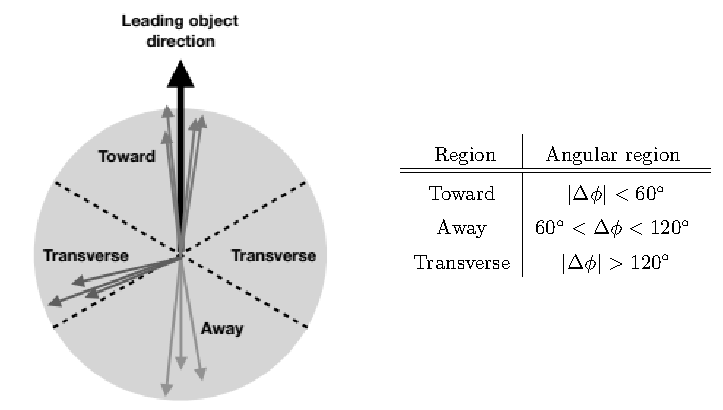
\includegraphics[width=0.8\textwidth]{{img/Regions.pdf}}
	\caption{This figure shows the four regions for the description of the UE on an event-by-event analysis. The angular values, defining the four regions, are shown in the table. The regions are defined starting from the leading object direction. The toward and away regions contain most of the contribution from the hard scattering (e.g. in a $t\overline{t}$ production event the two quark $t$ are located in these regions); while the transverse region are the ones in between the two other regions, these are the most important for the study of the UE.}
	\label{fig:Regions}
\end{figure}
%
\\
The regions classification is shown in \figRef{fig:Regions}, we have:
\begin{itemize}
	\item \textbf{Toward region}: the region that contains the leading object, this region contains most of the particles produced by the hard interaction.
	\item \textbf{Away region}: this region contains the objects that recoil against the leading object, also this region contains mostly the particles produced by the hard interaction.
	\item \textbf{Transverse regions}: the two transverse regions are the most sensitive to UE.
\end{itemize}
The toward and away regions are the ones with the major contribution from the primary hard scattering, in fact in a dijets event the leading jet is expected in the toward region while the next-to-leading jet in the away region.  
\\
The two transverse regions are called:
\begin{itemize}
	\item[--] \textbf{TransMAX}: This is the transverse region that contains the \textit{maximum} number of charged particles, or scalar $p_T$ sum of charged particles. This region includes both MPI and hard-process contamination.
As an example, in events with 3-jets production this region can contain the extra jet.	
	\item[--] \textbf{TransMIN}: is the transverse region that contains the \textit{minimum} number of charged particles, or scalar-$p_T$ sum of charged particles. This region is the most  sensitive to MPI effects.
\end{itemize}

\noindent The leading object definition depends on the type of event under observation and defer from one analysis to another. 
The charged-particle with the largest $p_T$ \cite{CMS-PAS-FSQ-15-007}, the dilepton system in Drell-Yan observation \cite{CMS:2012oqb, CMS:2017ngy} or $t\overline{t}$ events \cite{CMS:2018mdd} can all be used as the leading object in the analyses for the UE event.
\\
So we are interested in studying the transMAX and transMIN regions in particular the observable sensitive to UE in these regions. The main observables studied in these regions are the charged-particle density and the charged-particle scalar-$p_T$ sum density in the $\eta-\phi$ space.



\subsection{Hard scale dependence}

In a hadron-hadron collision with two jets productions, it is observed that not only the toward and away regions' activity increases with the hardness of the collision ($p_T^{max}$) but also the transverse regions' activity increases with it. This is shown in \figRef{fig:UEpredictions_in_regions.png}, where the different color lines refer to different scales for the collision. It is observed that the away region ($60\leq |\Delta\phi|\leq 120$) at increasing energy for the collision become broader this is related to the increasing quantity of FSR.
\\
This increment in the transverse regions activity cannot be explained only by the increase of the FSR. To explain this rise one needs to attribute activity in the transverse regions to MPI: the number of extra scatters increases with energy. This rise is related to the density functions for the partons inside the hadrons that increase when probed at higher energies and so the partons become denser packed in hadrons. In this way, the  probability of extra scatterings is larger to higher energies. 

\begin{figure}[!htb]
	\centering
	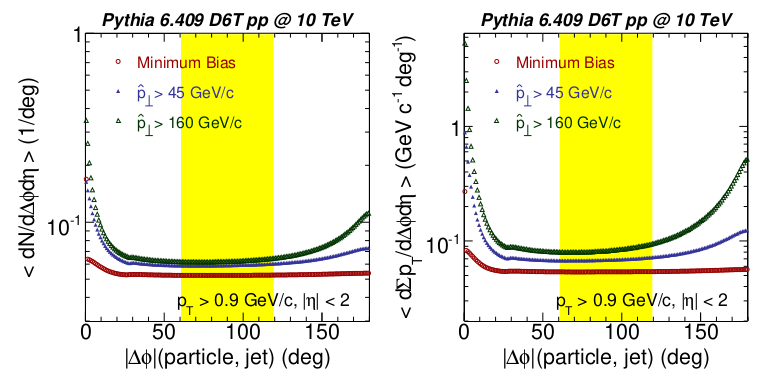
\includegraphics[width=0.8\textwidth]{{img/UEpredictions_in_regions.png}}
	\caption{A comparison between three different scales for the interaction, in \textsc{pythia}. The multiplicity of charged particles (left) and the scalar-$p_T$ sum of charged particles (right) are simulated. The activity in the transverse regions increase due to two effects: the FSR is related to the broadening of the away region so some events from the shower end up in the transverse region (yellow band) but this alone can't explain the increment so is required the introduction of the MPI in the description. Figure from chapter 5 of \cite{Bechtel:2009zza}.}
	\label{fig:UEpredictions_in_regions.png}
\end{figure}

\noindent The evolution of these two quantities in the transMAX region as a function of the transverse momentum of the leading object (measurement of the energy scale for the collision) is shown in more detail in \figRef{fig:CPtransmax_evolution_with_energy}. The two distributions show a rapid rise at low leading-object $p_T$ than a very low rise starts.
%
\begin{figure}[!htb]
	\centering
	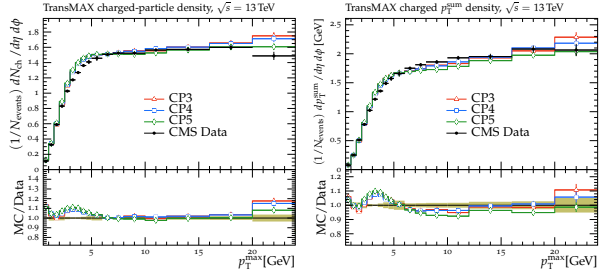
\includegraphics[width=0.9\textwidth]{{img/CPdistributions.png}}
	\caption{The evolution of the charged-particles density (left) and of the scalar-$p_T$ sum density of charged particles (right) as a function of the energy scale for the scattering (leading object $p_T$), the two distribution increase quite rapidly in the first bins than they saturate ($\approx 6-7\ \mathrm{GeV}$) the scalar-$p_T$ sum density increase a little bit more, for $p_T>$ but very slowly. The black dots are the experimental point and are compared to prediction with CMS \textsc{pythia} tunes: CP3, CP4 and CP5; they are described in more detail in the next chapter. Figure from \cite{CPtunes}.}
	\label{fig:CPtransmax_evolution_with_energy}
\end{figure}

\subsection{Sensitivity to MPI parameters}

Now we want to look for the sensitivity of these observables to some \textsc{Pythia8} parameters. \figRef{fig:CP5onlyPT0} shows the effect of the MPI on both the distributions shown before separately for TransMAX and TransMIN regions. 
%The amount of the MPI is related to the value of $p_{T0}$: an high value of $p_{T0}$ is related to less MPI (blue line) and an higher value to a major contribution from the the MPI (red line).
The figure shows the case with MPI (red line) and the case when the MPI are switched off (blue line). As expected the MPI are needed to explain the activity in the transverse regions. When the MPI are switched on the number of particles produced is higher than the case when they are off. From this figure is clear that MPI are the main contribution to the activity of these TransMAX and TransMIN regions. Obviously, the discrepancy increases as the hard scale of the interaction increases, in fact in low $p_T$ regions the $p_T$ evolution starts at a lower value so the phase-space, for the extra collisions to occur, is smaller.


\begin{figure}[!htb]
	\centering
	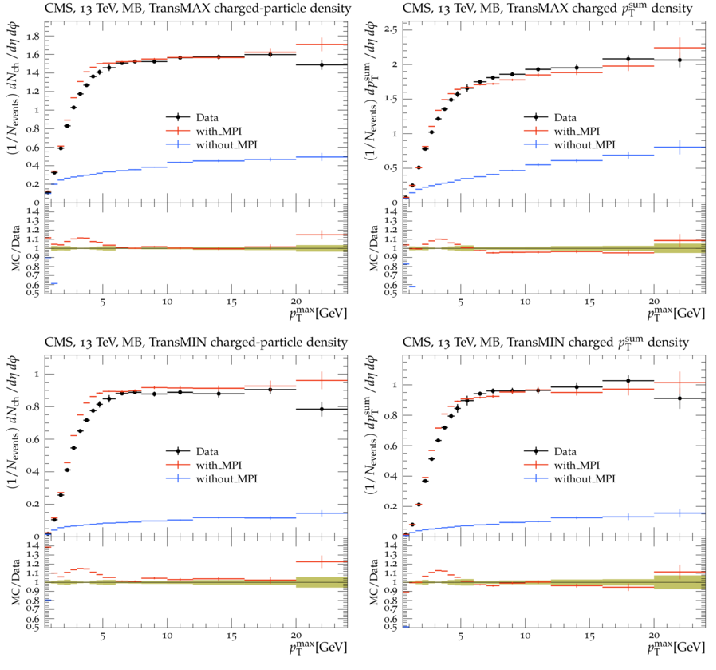
\includegraphics[width=0.9\textwidth]{{img/CP5_with_without_MPI.pdf}}
	\caption{This image shows the effect of the MPI in the transMAX and TransMin regions. The contribution of the parton shower alone can't explain the contributions of the underlying event in these two regions (blue line) the introduction of the contribution from the MPI is necessary (red line). The two simulations are compared to the data from \cite{CMS-PAS-FSQ-15-007}.}
	\label{fig:CP5onlyPT0}
\end{figure}

Another important observation that was also pointed out in the \chapRef{sec:BasicConcepts} is that the amount of activity in the two transverse regions is also dependent on the center-of-mass energy. This evolution is shown in \figRef{fig:CPECMdep} for two different energy. The amount of MPI increase with $\sqrt{s}$ that was expected from the evolution of the PDF with the energy of the collision: the hadrons become denser-packed when probed to higher energies. In \figRef{fig:CPECMdep} the charged particle density and the scalar sum of the transverse momentum in the transverse regions data are compared for two different center-of-mass energies. The data are also compared to existing different CMS tuning.

\begin{figure}[!htb]
	\centering
	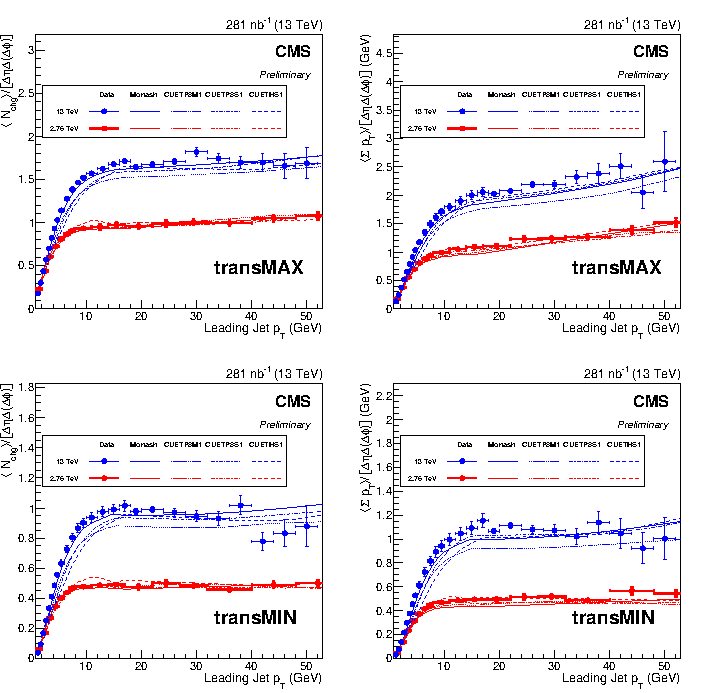
\includegraphics[width=0.9\textwidth]{{img/CPECMdep.pdf}}
	\caption{The charged particle density in the transMAX (upper left) and transMIN (lower left) regions and of the charged particle $p_T$-sum in the transMAX (upper right) and the transMIN (lower right) regions evolution as function of the center-of-mass energy is shown. The red ones are the data for $\sqrt{s}=2.76$ and the blue ones for $\sqrt{s}=13$ and these are compare to different CMS tunes. Figure from \cite{CMS-PAS-FSQ-15-007}}
	\label{fig:CPECMdep}
\end{figure}

So these observables are the main ones we are going to use in our tune and used in previous tunes for the UE. The data from the activity in the TransMAX and TransMIN  regions have been collected by  a large number of experiment at different center-of-mass energies. 

The selection criteria for CMS data from analyses \cite{CMS-PAS-FSQ-15-007} and \cite{CMS-PAS-FSQ-12-020} are the selection of charged particle tracks within the pseudorapidity range $|\eta| < 2$ and $p_T \geq 0.5\ \mathrm{GeV}$ in order to ensure a good track reconstruction efficiency. Fake tracks after mis-reconstruction are removed imposing to pass the \textit{highPurity} \cite{HighPurity}. Secondary decays are removed by requiring the impact parameter significance $d_0/\sigma_{d\,0} < 3$ and the significance in the z-direction $d_z/\sigma_{d\,z} < 3$. Then to keep only tracks with good resolution the tracks with relative uncertainties $\sigma_{p_T}/p_T > 0.05$ are discarded.
\\
To reconstruct the charged particle jets the clustering algorithm use is the Seedless Infrared-Safe Cone (SISCone) \cite{JetAlgorithm1} jet algorithm\footnote{The the Anti$-k_T$ algorithm \cite{JetAlgorithm2} is currently the more preferred jet clustering algorithm in CMS but to ensure continuity with respect to the previous analyses on the UE the one above is chosen.}. Charged particle within the pseudorapidty range $|\eta|<2.5$ are used for jet reconstruction then the reconstructed jet have to pass the above selection criteria.
\\
Minimum bias events are triggered by requiring activity in both Beam Scintillator Counters (BSC) located at a distance of $\pm10.86\ \mathrm{m}$ from the detector center and are sensitive within $3.23 < |\eta| < 4.65$ in coincidence with signals from both beams in the Beam Pick-up Timing for eXperiments (BPTX) devices these coincidence indicate that both the beams are crossing at the same time and that they interact.
 

\subsection{Observables in Z production processes}

In the last part of this work, it will performed the tune of primordial $k_T$ another important parameter in the simulation of hadron-hadron collisions. An unresolved question is that the primordial $k_T$ value required for the description of the observed cross-section for the Z production is very large with respect to the expected value derived from the typical size of a hadron in \eqRef{eq:PrimordialKT}. This very high value is not understood by first principles so it is required a tune for this parameter in the Monte Carlo generator in order to describe the data in a good way. 
\\
The observables to study the primordial $k_T$ are the differential cross-section for Z production in proton-proton collision in Drell-Yan observation as a function of the transverse momentum of the Z boson (\figRef{fig:PrimordialkT_distributionUsed_noFxFx} left) and as a function of the $\phi^*_\eta$ angle (\figRef{fig:PrimordialkT_distributionUsed_noFxFx} right). Where the angle $\phi^*_\eta$ is defined as:
\begin{equation}
	\phi_\eta^*=\tan\left(\frac{\pi-\Delta\phi}{2}\right)\,\sin(\theta_\eta^*)\quad,
	\label{eq:def_phistar}
\end{equation}
where $\Delta\phi$ is the azimuthal angle between the two leptons. The angle $\theta_\eta^*$ instead is the angle measured with respect to the beam direction in the rest frame of the dilepton system (frame with leptons emitted back-to-back), so is defined as: 
\begin{equation}
	\cos(\theta_\eta^*)=\tanh\left(\frac{\eta^--\eta^+}{2}	\right)\quad,
\end{equation} 
with $\eta^+$ and $\eta^-$ the pseudorapidities of the two leptons \cite{phistareta}.

\begin{figure}[!htb]
	\centering
	\noindent
	\begin{subfigure}{0.5\textwidth}
	\centering
	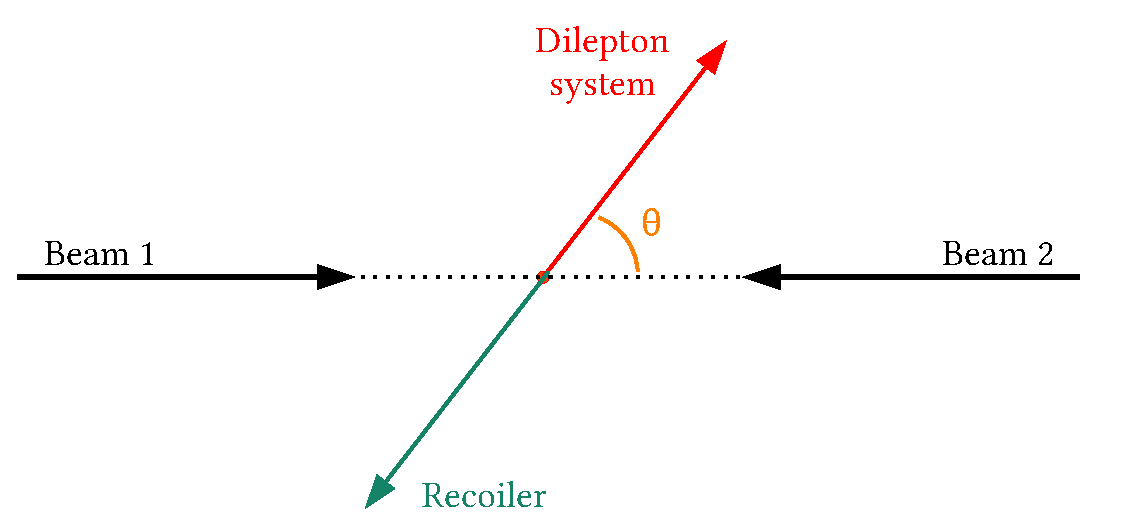
\includegraphics[width=0.97\textwidth]{{img/Angle1.pdf}}
	\end{subfigure}%
	\begin{subfigure}{0.5\textwidth}
	\centering
	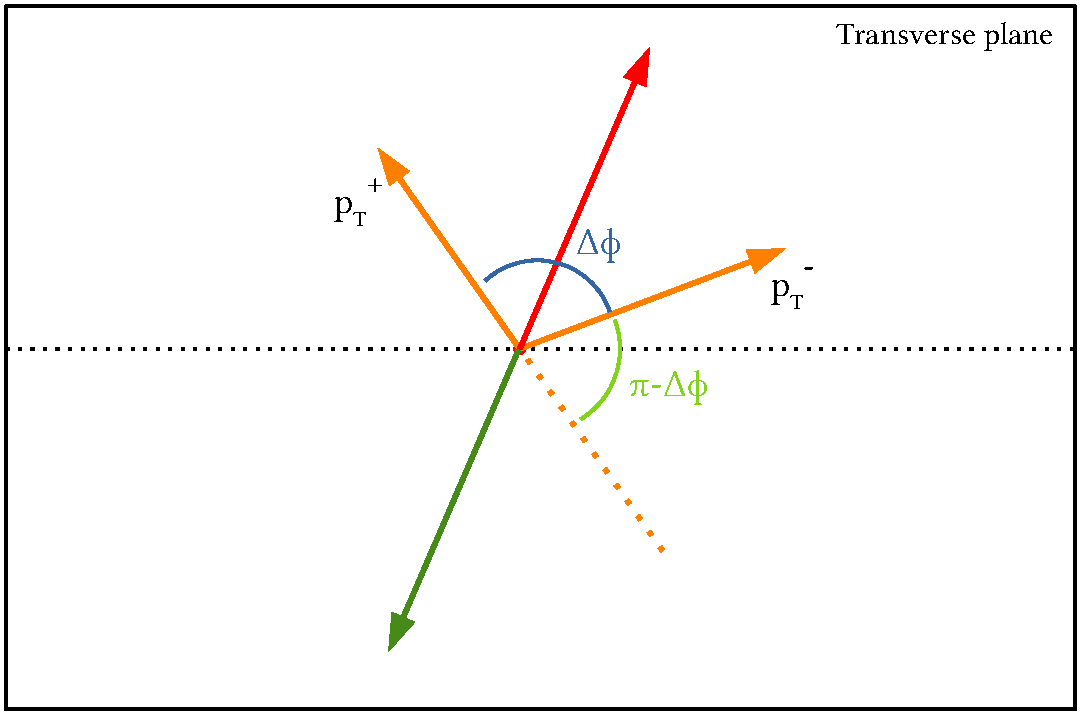
\includegraphics[width=0.97\textwidth]{{img/Angle2.pdf}}
	\end{subfigure}
	\caption{A schematic representation of a Drell-Yan observation with a description of the angles used in the definition of $\phi_\eta^*$ in \eqRef{eq:def_phistar}. }
	\label{fig:angles}
\end{figure}

The $Z$ boson is a very massive boson,$m=91.1876 \pm 0.002\ \mathrm{GeV}$ \cite{PDG}, which can be produced only in the hard  scattering of two partons of the hadron undergoing the collision, then after a very short lifetime the $Z$ boson decay in a couple of leptons: $e^+\,e^-$ or $\mu^+\,\mu^-$. The measurement of this final state takes information on the $Z$ boson that is not directly observed by experiments. 
It is a matter of fact that the production of the $Z$ boson can be affected by all the other soft processes taking place along with this production that can change the topology of the initial state. In the last chapter it is investigated the effect of ISR and Primordial $k_T$ on the $Z$ boson production in the low region of the spectrum.  
\\
Since the $Z$ boson production is a hard process to full simulate the Z production spectrum we have to merge matrix element calculation and space shower to do this we have to use a margin scheme. To have a good description of the high region of the spectrum ($p_T^Z > 2\ \mathrm{GeV}$) we have to include higher-order calculation to consider NLO and NNLO processes and so we have to adopt a more complex merging scheme as the FxFx merging scheme that has been introduced in \chapRef{chap:Hadron-HadronScattering}. 
\\
As shown in \figRef{fig:PrimordialkT_distributionUsed_noFxFx} the description at LO (and without the need for FxFx) is good only in the first bins that are the ones of interest for the study of underlying event effects and it is less computationally expensive than running all the FxFx merging scheme. So, the strategy followed for the tuning of the primordial kT in the \chapRef{chap:primordialkTtune} is to tune the Primordial $k_T$ in this low region, the one of interest, taking only the first 5 bins from each distribution.
\\
Then the full simulation with FxFx is run only for the comparison once the parameters have been tuned. This is going to be discussed in more detail in \chapRef{chap:primordialkTtune} where the primordial $k_T$ tune is performed.

\begin{figure}[!htb]
	\centering
	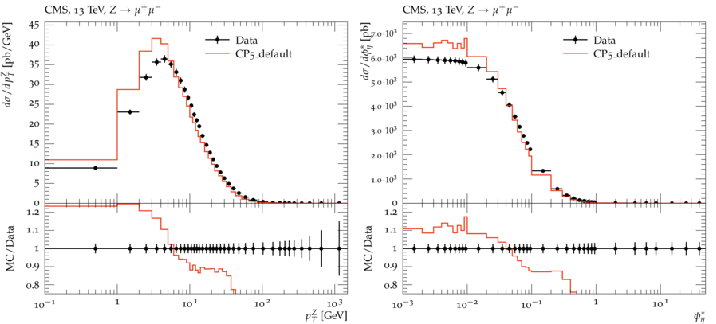
\includegraphics[width=0.9\textwidth]{{img/PrimordialkT_distributionUsed_noFxFx.pdf}}
	\caption{Here are shown the distribution, from the \cite{ZpT_distributions} CMS analysis at $\sqrt{s}=13\ \mathrm{TeV}$, which we are going to use for the tune of the primordial $k_T$. The left one is the $Z$ boson production cross-section as a function of the transverse momentum of the $Z$ boson. On the right the differential cross-section for the $Z$ boson production as a function of the $\phi_\eta^*$ angle. The red line is the \textsc{pythia8} description before the tune of the primordial $k_T$ and without the FxFx merging scheme so only the first bins have to be taken into account.}
	\label{fig:PrimordialkT_distributionUsed_noFxFx}
\end{figure}


In the following section, we will introduce the existing CMS tunes for the  UE in minimum bias observations. These tunes are able to reproduce very well the observables described in \secRef{sec:Minimum Bias Measurements and Underlying Event topology} at $1.96$, $7$ and $13\ \mathrm{TeV}$. 
%But as we are going to see in \chapRef{chap:Hadron-HadronScattering} the tunes do not describe well the low region of the $Z$ boson production cross section so a further tune on these observable is performed.


\section{Previous Tune for the Underlying Event}

In the paper \cite{CPtunes} the CMS collaboration presents new \textsc{pythia8} tunes for the underlying event (UE). The tunes are called CP and a number from 1 to 5 where CP stands for \textsc{"cms pythia8"}. The tunes are performed by changing the values of the coupling constant $\alpha_s$ for the ISR, FSR, hard scattering and MPI and changing the order of the evolution for the $\alpha_s$ with the $Q^2$ value of the interaction. Another difference among these tunes is the choice of the PDF set: CP1 and CP2 use a LO PDF, CP3 an NLO one, while CP4 and CP5 tunes use an NNLO PDF set. 

The tuned parameters are shown in \tableRef{table:CP5variations} with the associated variation ranges and a recall of the definition of each one. 
\begin{table}[H]
	\centering
	\resizebox{0.97\textwidth}{!}{
	\begin{tabular}{l c c}
		Parameter description & Name in PYTHIA8 & Range considered\\\hline\hline
		\\[-8pt]
		MPI threshold $[\mathrm{GeV}]$, \texttt{pT0Ref}, at $\sqrt{s}=\sqrt{s_0}$ \ & \texttt{MultipartonInteractions:pT0Ref} &  $1.0-3.0$ \\[3pt]
		Exponent of $\sqrt{s}$ dependence, $\epsilon$ & \texttt{MultipartonInteractions:ecmPow} & $0.0-0.3$ \\[3pt]
		Matter fraction contained in the core & \texttt{MultipartonInteractions:coreFraction} & $0.1-0.95$ \\[3pt]
		Radius of the core & \texttt{MultipartonInteractions:coreRadius} & $0.1-0.8$ \\[3pt]
		Range of color reconnection probability & \texttt{ColorReconnection:range} & $1.0-9.0$ \\[3pt]
	\end{tabular}
	}
	\caption{This table reports the five parameters tuned for the UE and Minimum Bias in CP* tunes, the variation ranges used for the sampling are shown in the last column. Table from \cite{CPtunes}}
	\label{table:CP5variations}
\end{table}

\noindent These parameters are the ones that govern the number of MPI and the amount of Color Reconnections\footnote{Note that all the other parameters are set to the default values of the Monash tune \cite{Monash}}. These CP* tunes want to be general (multi-purpose) tunes for UE and minimum bias observables described above.

These tunes are performed with the standard tool for the  high energy physics tune: \textsc{professor}. 



\subsection{The distributions used for the Tune}
\label{sec:Thedistributionsused}

The observables distributions used for the tune are the following ones:

%\begin{table}
%	\centering
%	%\resizebox{\textwidth}{!}{
%	\begin{tabular}{l l}
%	Rivet Analysis & Distribution\\\hline\hline
%	\\[-8pt]
%	CMS\_2015\_I1384119 & d01-x01-y01\\[2pt]
%	CMS\_2015\_PAS\_FSQ\_15\_007 & d01-x01-y01\\[2pt]
%	CMS\_2015\_PAS\_FSQ\_15\_007 & d02-x01-y01\\[2pt]
%	CMS\_2015\_PAS\_FSQ\_15\_007 & d05-x01-y01\\[2pt]
%	CMS\_2015\_PAS\_FSQ\_15\_007 & d06-x01-y01\\[2pt]
%	CMS\_2012\_PAS\_FSQ\_12\_020 & d05-x01-y01\\[2pt]
%	CMS\_2012\_PAS\_FSQ\_12\_020 & d06-x01-y01\\[2pt]
%	CMS\_2012\_PAS\_FSQ\_12\_020 & d08-x01-y01\\[2pt]
%	CMS\_2012\_PAS\_FSQ\_12\_020 & d09-x01-y01\\[2pt]
%	CDF\_2015\_I1388868 & d01-x01-y01\\[2pt]
%	CDF\_2015\_I1388868 & d02-x01-y01\\[2pt]
%	CDF\_2015\_I1388868 & d05-x01-y01\\[2pt]
%	CDF\_2015\_I1388868 & d06-x01-y01\\[2pt]
%	CMS\_2018\_I1680318 & d01-x02-y01\\[2pt]
%	CMS\_2018\_I1680318 & d01-x03-y01\\
%	\end{tabular}
%	%}	
%\end{table}

\begin{itemize}
	\item The pseudorapidity distribution of charged hadrons ($p$, $K$ ,$\pi$) measured for an
inclusive selection in inelastic proton-proton collisions \cite{CMS:2015zrm}; 
\item Charged particle density and charged particle scalar $p_T^{sum}$ in TransMIN and TransMAX regions at different $\sqrt{s}$ ($1.96\ \mathrm{TeV}$ \cite{CDF:2015txs}, \, $7\ \mathrm{TeV}$ \cite{CMS-PAS-FSQ-12-020}, \, $13\ \mathrm{TeV}$ \cite{CMS-PAS-FSQ-15-007});
\item The pseudorapidity distributions for single diffractive (\textsc{sd}) and non single diffractive (\textsc{nsd}) events selection \cite{CMS:2018nhd}.
\end{itemize}
In the next chapter, we will describe our tune using \textsc{mcnntunes} and in it we used the same distribution listed here. All the graphs for these observables are then shown with the final tunes descriptions.



\subsection{Pyhtia configuration and the tunes}

On the top section of \tableRef{fig:CPtunes1} and \tableRef{fig:CPtunes2} are reported the values for the \textsc{pythia8} parameters used in the CP tunes and, on the bottom, the five parameters resulting from the tune.
\begin{table}[!htb]
	\centering
	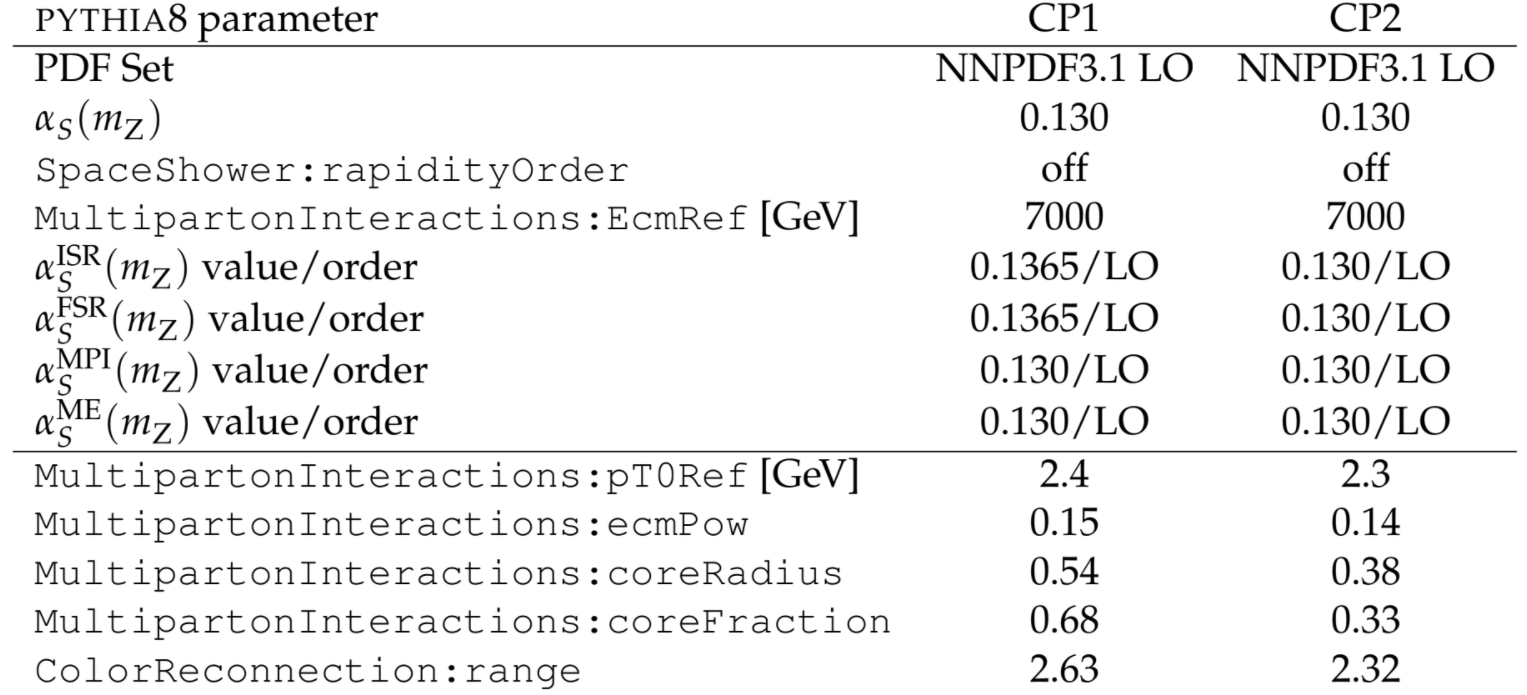
\includegraphics[width=0.95\textwidth]{{img/CPtunes1.png}}
	\caption{CP1 and CP2 tunes settings are reported here together with the values for the parameters tuned. CP1 and CP2 use a LO PDF set. CP1 $\alpha_s$ is different between matrix element calculation and MPI that use a value of 0.1365 ISR and FSR that instead uses 0.130. While CP2 use the same value for all processes, it is fixed at 0.130. In both cases $\alpha_s$ run with a LO evolution. Table from \cite{CPtunes}}
	\label{fig:CPtunes1}
\end{table}
\begin{table}[!htb]
	\centering
	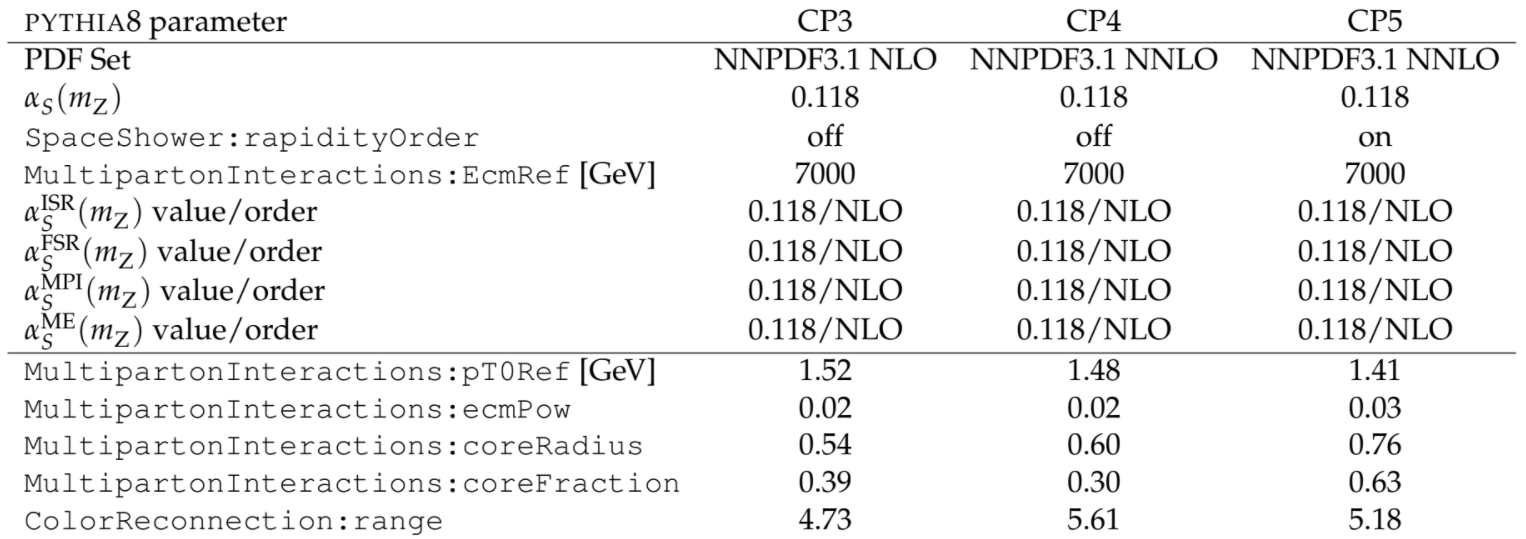
\includegraphics[width=0.95\textwidth]{{img/CPtunes2.png}}
	\caption{Here are reported CP3, CP4 and CP5 tunes settings, and the results for the tune. The three tunes use an equal $\alpha_s$ value for all the processes, $\alpha_s=0.118$ running with a NLO evolution. The difference between CP3 and the other two tune is that CP3 use an NLO PDF set while CP4 and CP5 an NNLO one. CP5 ISR emission is also ordered according to rapidity. Table from \cite{CPtunes}}
	\label{fig:CPtunes2}
\end{table}
\\
Below we are going to focus on the CP5 tune. We are going to reproduce this tune using the same settings for \textsc{pythia8} but using a different tuning software: \textsc{mcnntunes}. 
\\

%%%% INTRODUCTION to the next chapter

\medskip

The next chapter discusses the general approaches to the tune and why we use machine learning and on the description of the main tool used for the tuning in this work \textsc{mcnntunes}. 
%\textsc{mcnntunes} is also introduced together with the already existing CP* tunes in particular the CP5 tune.
